\documentclass[10pt]{article}
\usepackage{latexsym}
\usepackage{natbib}
\usepackage{graphicx}
\usepackage{subfigure}
\usepackage{listings}
\usepackage{algorithm}
\usepackage{algpseudocode}

\title{Homework 1: Eigendigits}
\author{Shun Zhang}
\date{}

\begin{document}
\maketitle

\section{Introduction}

In this report, I applied principal components analysis on digits
classification problem. 60000 training samples and 10000 testing
samples are provided.

Eigenvectors on first 2000 training samples.

\begin{figure}[b]
\centering
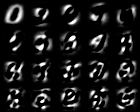
\includegraphics[]{eigen.png}
\caption{First 20 eigen-vectors, aligned from left to right and top to
down. Each value is multiplied by 10, i.e., each vector has norm of
100, instead of 1. They become dark after normalization.}
\label{fig:eigen}
\end{figure}

Reconstructed digits using first 100 and 200 eigenvectors
correspondingly. First 2000 training samples are used. 

\begin{figure}[b]
\centering
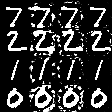
\includegraphics[]{test.png}
\caption{Reconstruction of digits. From left to right on each line,
there are original digits, digits constructed by first 100
eigenvectors, digits constructed by first 200 eigenvectors, digits
constructed by first 600 eigenvectors. }
\label{fig:test}
\end{figure}

\section{Experiments}

On different size of data.

%hw1Classify(n, 1000, 200, 1)
\begin{figure}[b]
\centering
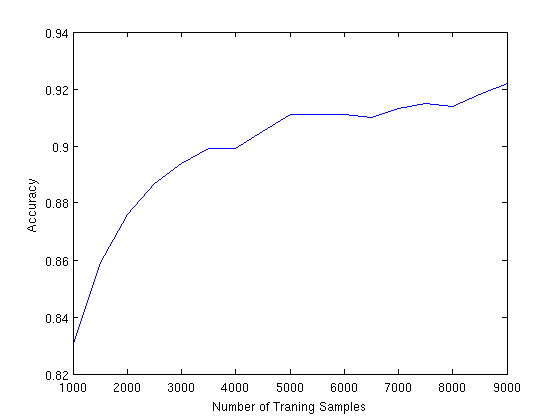
\includegraphics[width=0.8\columnwidth]{diffDataSet.png}
\caption{Comparison on using different number of training samples.
Testing on first 1000 testing set. Using first 200 eigen-vectors. K
for K-nearest-neighbors is 1.}
\label{fig:dataset}
\end{figure}

Using different number of eigenvectors.

\begin{figure}[b]
\centering
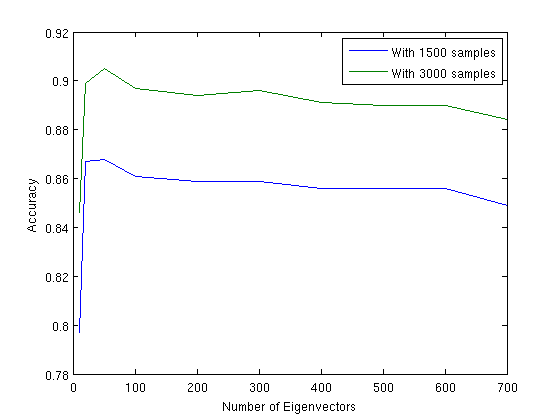
\includegraphics[width=0.8\columnwidth]{diffEVector.png}
\caption{Comparison on using different number of eigenvectors.
Testing on first 1000 testing set. Using first 1500 and 3000 training
samples for each line.  K for K-nearest-neighbors is 1.}
\label{fig:evec}
\end{figure}

\end{document}
